% The first command in your LaTeX source must be the \documentclass command
%\documentclass[acmsmall, nonacm, 10pt]{acmart}
\documentclass[10pt, titlepage]{article}

% Use bibtex
\usepackage{cite}
\usepackage{url}

% Make bib style "proper"
\usepackage[square,numbers]{natbib}

% Package for code snippets
\usepackage{xcolor}
\definecolor{code-bg}{rgb}{0.9725, 0.9725, 0.9725}

\usepackage{minted}

\setminted{
	%frame=lines,
	%framesep=2mm,
	baselinestretch=1.2,
	fontsize=\small,
	linenos=true,
	xleftmargin=20pt,
	bgcolor=code-bg,
	tabsize=2,
	obeytabs=true,
	showtabs=false
}

\BeforeBeginEnvironment{minted}{\smallbreak}
\AfterEndEnvironment{minted}{\smallbreak}

\usemintedstyle{emacs}
\usepackage{listings}

% Make links
\usepackage{hyperref}
\hypersetup{
    colorlinks,
    citecolor=black,
    filecolor=black,
    linkcolor=black,
    urlcolor=black
}

% Packages to set graphics and float spacing
\usepackage{graphicx}
\usepackage{float}

% Math symbols and math
\usepackage{amsmath}
\usepackage{amssymb}

% Set required line spacing to double
\usepackage[onehalfspacing]{setspace}

% Fix margins to 1 inch
\usepackage[a4paper,margin=1in,footskip=0.25in]{geometry}

% Set headers to all be left aligned
\usepackage[raggedright]{titlesec}

% Change paragraphs to no indent
\setlength\parindent{0pt}

% begin document
\begin{document}

% Set article title
\title{Attacking WEP By Exploiting IV Selection}


% builds the header section with title, names, student numbers...
\begin{titlepage}
	\centering
	\vspace{3cm} \par
	\huge Attacking WEP By Exploiting IV Selection \par
	\large Exploiting the 24-bit IV in WEP for network authentication by simulating high volumes of traffic\par
	\vspace{8cm} \par
	Tyson Steele - 101000208\\
	Ryan Kane - 101041831\\
	Neilesh Chander - 101040037
	\vfill
	% Page footer
	\large Carleton University \par
	\large \today\par
\end{titlepage}
\newpage

% Build table of contents
\tableofcontents
\newpage

% Build list of figures 
\listoffigures
\newpage

% Build list of tables
\listoftables
\newpage

% --------------------------------------------- Main Body -------------------------------------------- %
\section{Introduction}

\subsection{Project Domain}
Wi-Fi is a crucial part of today’s lifestyle, used everywhere from personal homes to businesses. Since Wi-Fi is a wireless technology there is no inherent security built-in. Wired Equivalent Privacy (WEP) is an algorithm that was developed to ensure that wireless networks had similar security and confidentiality to wired ones. To this day there are still networks that rely on the security WEP provides. WEP uses the RC4 stream cipher and the CRC checksum with a 40-bit or 104-bit key. The RC4 cipher uses an IV to randomize the key, however this IV is only 24-bits. This limitation means that on a busy network the key could be repeated, leading to it being known.

\subsection{Purpose}
This paper aims to look at the WEP protocol and how, even though it is still used to this day, it has serious security flaws that can expose the network key. With the use of such a small initialization vector (24-bit) a busy network has a 50\% chance of repeating the same IV after roughly 5000 packets have been sent. This leads to a 50\% chance of recovering the key after 40 000 packets have been sent, and increases to 95\% after 85 000 packets. With the network key it then becomes trivial to authenticate to the network and gain potentially unauthorized access to systems.

\subsection{Motivation}
Given that WEP was a widely used protocol in wireless networks, it is interesting to learn about a massive security flaw that affects it. There are even some devices currently using WEP which makes the attack that we use in this paper even more relevant. Most devices that people use everyday connect over wireless networks, but often people do not check the protocol that their network is using and just trust that it is secure. This project is an opportunity to learn about how protocols like WEP work, and learn about ways that they can be exploited to better our understanding of how the security in the networks we use are fallible. This project also provides an opportunity to work with open source network security tools that are used in real world settings to test and break network protocols.




\section{Background}
\subsection{RC4}
RC4 was one of the most commonly used stream ciphers. Originally a proprietary algorithm, the inner workings were not made public, making security research and verification very difficult. For a long time many use cases assumed blind trust in RC4. It was reverse engineered in 1994, which led to the discovery of its weakness. Before this discovery, RC4 was used for an approximated 50\% of TLS traffic, as well as for WEP, WPA, PDF, BitTorrent, and MS Point-To-Point Encryption. RC4 is fast, easy to implement, and allows variable key lengths \cite{appliedCrypto}. This allows it to easily be used on machines with relatively low computational resources, extending usability across the maximum number of systems. However, these same reasons as well as the fact that RC4 does not implement a nonce eventually lead to the discovery of fundamental flaws in RC4 that can be exploited, consequently resulting in RC4 no longer being considered secure. Unlike RC4, modern stream ciphers use a nonce in order to gain randomness in case the key is reused, increasing the security of the cipher.

\subsection{Advanced Encryption Standard (AES)}
AES Replaced DES as the standard for block ciphers in 2001. DES used a 56 bit key to encrypt blocks of 64 bits by taking the plaintext and passing it through an initial permutation then running a 16 round Feistel cipher; each generating a new 48 bit key to be used. Contrary to RC4, DES has become outdated due to the small block and key sizes rather than design flaws. By using a small 56 bit key, DES could be brute forced in $2^{56}$ steps. Brute force attacks are computationally intensive, so alone this would not be cause for major concern; however, by 2000, attacks monitoring differential power usage analysis could identify the key after 100 encryptions, and today there exists specialized hardware designed to recover the key in less than 24 hours. \\

AES was a major advancement over DES as it was modern, and did not contain known vulnerabilities that could be abused by private agencies such as the NSA. AES is built up from many rounds of substitution-permutation network instead of Feistel ciphers. "AES is as secure as a block cipher can be..." \cite{appliedCrypto}. We can't say it will never be broken; however, to this day no vulnerabilities or weaknesses have been found. AES uses a block length of 128 bits along with either a 128 bit key and 10 rounds, 192 bit key with 12 rounds, or a 256 bit key with 14 rounds to obfuscate the plaintext message into ciphertext that cannot easily be reversed. \\

% ADD PICTURE HERE ??
%\begin{figure}[H]
% 	\centering
%    \includegraphics[width=0.5\textwidth]{./images/aes-visual.png}
%    \caption{AES Workflow}
%\end{figure}

While the AES that is used in practice has not been broken, it is common to attack weaker versions of encryption schemes in order to get insight as to how stronger versions can potentially be compromised \cite{appliedCrypto}. Known AES attacks on reduced versions have broken a 128 bit key with 7 rounds out of 10, 192 bit key over 8 rounds out of 12, and 256 bit key over 9 rounds out of 14 \cite{appliedCrypto}. \\

Since AES has currently not been compromised, it is still safe to be used today, and can be found in recent networking standards such as WPA2/WPA2-PSK.

\subsection{WEP and WPA2/WPA2-PSK}
We know that an encryption scheme can only be as secure as the underlying ciphers it is based on. WEP implements RC4 which we now know to be completely insecure, this is why we are able to easily crack WEP by attacking the underlying RC4 components. Similarly, since AES has not been broken, WPA2 and WPA2-PSK (pre shared key) are still considered safe, although as consumer hardware continues to increase in power,  we are beginning to shift towards stronger encryption schemes Salsa/ChaCha, and other elliptic curve methods. \\

\subsection{WEP Problems}
WEP relies on RC4, and as a result has many inherent problems that make the wireless protocol totally insecure. This includes easily finding collisions, using decryption dictionaries if storage is available, using message modification,  and authentication spoofing. WEP uses a 24 bit IV ($v$) and a 32 bit checksum of message m to send a ciphertext ($c$) over the network. The checksum is referred to as $c(m)$, and ciphertext $c$ is computed as $RC4(v,k) \oplus <m || c(m)>$. Resulting in a packet being sent in the format $v || c$. Messages are received and decrypted by first computing $RC4(v,k)$, accepting the message if the decrypted plaintext and checksum are valid. \\

Collisions are very easy to find, since $RC4(v,k)$ relies on $v$ and $k$ where $k$ is a secret key that rarely changes, and is commonly shared between everyone connected to the network. This reduces the complexity of cracking to be finding $v$, which will have a guaranteed collision after approximately 16 million collisions ($2^{34}$). If $v$ is chosen randomly, we can consider the birthday problem in order to estimate the amount of attempts before a collision is expected. This results in an expected $2^{12} = 4096$ transmissions before a collision. However, for wireless implementations, it is common to start with $v= 0$, and increment after each transmission, therefore we expect a higher number of collisions when $v$ is small. Since the value of $v$ is sent during the transmission, this can constantly be checked by an attacker. \\

Using a known plaintext attack by monitoring packets before they are sent, we know the corresponding RC4 output. Creating known network traffic by creating packets or constantly running network operations until a collision on v is observed. Once this occurs, an attacker can decrypt both plaintexts from overlapping keys using the known plaintext, and create a comprehensive decryption dictionary. 



\section{Literature Review}
\subsection{Attacks on the RC4 Stream Cipher \cite{klein}}
This paper is the main paper that this project is based on. It proves a relationship between keystreams and the key in the RC4 algorithm. This relationship is the basis of the exploit that the attack in our project uses. 

\subsection{Breaking 104 Bit WEP in Less Than 60 Seconds \cite{mainPaper}}
This paper presents a full attack to retrieve the WEP key. It describes the method to capture a sufficient amount of keystreams and use them to get the key with an algorithm based on the exploit shown in Kleins paper. It uses an approximation of the formula that Klein presents to efficiently compute the key bytes in parallel as opposed to iteratively as Kleins formula does. Then it proves through simulations with the Aircrack library that the attack can be done with relatively low cost equipment very quickly. 

\section{Frameworks and Technologies}
In order to get the project to where it is, we had to use a multitude of existing libraries as well as existing tools. The entire project was written using the Python programming language, and a little bit of shell script to help automate the data collection process. In the Python code we used many libraries, the major ones being the scapy library to help construct the deauthentication packets, as well as send them. We also used the subprocess library to start, manage and stop the aircrack processes from within Python. The last major library used was the multiprocessing library. This library allowed us to run different aircrack modules simultaneously from the same Python program while individually managing them. \\

We also used the existing command line suite aircrack-ng. This suite packages a lot of useful tools, of which we used: airodump-ng to capture the packets being sent on the network, aireplay-ng to control the deauthentication packets we were sending as well as duplicating and injecting the ARP requests, aircrack-ng to apply Klein’s key ranking attack on the captured packets/IVs. During initial testing, WIreshark was used to capture packets on the network, as well as to analyze ARP packets to better learn their structure with the goal of being able to identify them when encrypted with WEP. In combination with this, a hex editor was used to attempt to manually modify packets to format them as required for re-injection (changing MAC address, sequence number, and recalculating the checksum).

\section{Methodology}
Before any code writing or program testing could be done, there needed to be a network to work off of. In order to accomplish this, an older D-Link router was used. It was connected to an existing local area network to allow internet access through. Navigating to the D-Link router portal at 192.168.0.1 allowed for the configuration of the network settings. Once there we were able to select WEP as the encryption method, choose the authentication type (basic/open) as well as the length of the key and the key itself (hackr). These settings can all be seen in the figure below.\\

\begin{figure}[H]
 	\centering
    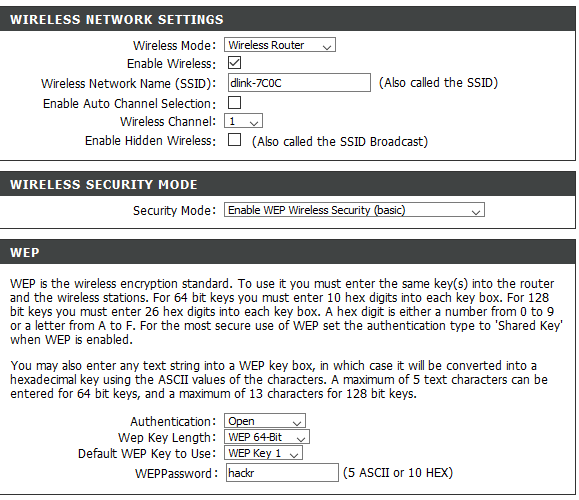
\includegraphics[width=0.5\textwidth]{./images/wep_settings.png}
    \caption{Router Configuration}
\end{figure}

Once the network was set up we needed a target device to simulate traffic, and a device to act as the attacker. A cell phone was used as the target device, and an old laptop running Linux was used as the attacker. This attacking device needed to be Unix based since Windows machines are usually unable to put the network interface card into monitor mode, which is required for capturing packets not destined for the network interface card. To get the laptop in monitor mode, we run the following commands.\\

\begin{minted}{bash}
sudo apt-get update
sudo apt-get install aircrack-ng -y
sudo airmon-ng check kill
sudo airmon-ng start <wireless_iface>
\end{minted}

The process for applying the attack is fairly straightforward. The attacker (laptop) needs to listen to traffic on the target network and capture as many unique IVs as possible. WEP will use a random IV, 24-bits in length, every time it encrypts a new packet. In most real cases there would be a lot of traffic on the network (perhaps a hotel), but in our case there was just the one device. So we needed to speed the process up by creating our own traffic. This was accomplished by repeatedly sending the router Address Resolution Protocol (ARP) requests, with which the router would duplicate by broadcasting, and the other device (the phone) would send an ARP reply. Therefore, with one packet being injected, two unique IVs were created. ARP was also chosen because they are at the Link Layer of the Internet Protocol (IP). Packets at such a low level are generally not rate limited since it is the hardware speaking. ARP packets also have a static data structure for the first 8 bytes (seen in Figure 2), with the only difference being a 0x01 for ARP request and 0x02 for ARP reply. This allows us to get a 16-byte partial keystream by XORing the plaintext ARP pattern (and the Logical Link Control header) with the encrypted equivalent.\\

\begin{figure}[H]
 	\centering
    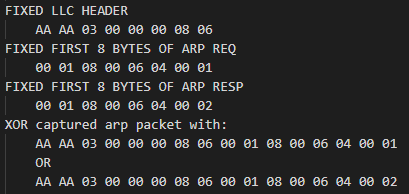
\includegraphics[width=0.5\textwidth]{./images/fixed-bytes.png}
    \caption{Fixed Bytes of LLC and ARP Packets}
\end{figure}

Once enough partial keystreams have been captured (1 keystream = 1 IV), a key ranking algorithm can be used to find the correct key (given enough of them). 

\subsection{Key Ranking Algorithm (PTW)}
Tews et al. then describes an algorithm for determining the correct key based on the input of the collected keystreams \cite{mainPaper}. Each byte in the key is approximately computed using every recovered byte from the keystream and a modified version of the formula presented in Kleins paper. Each time the key byte is approximated using a key stream, the value that is computed is voted for as the correct key byte. The votes are tracked for every key byte and the value with the highest vote at the end is assumed to be the correct key byte. Using the modified approximate calculation, the key bytes can be computed this way in parallel instead of iteratively as in Klein's solution.\\

If the sample size is small, the correct key byte may not be the one with the highest number of votes. Initially, the algorithm selects each key byte that has the highest number of votes and determines if that key is correct. If it is not, the algorithm selects the next closest key byte by votes out of all the key bytes and adds that single key byte into the key bytes that have been selected. Everytime the algorithm selects a new key byte this way, it checks all the new possible combinations of key bytes out of the ones that have already been selected. The algorithm repeats this process until the correct key is found. \\

There are certain cases where the modified approximation used to calculate the key byte does not get the correct key byte. In this case the approximation will not render the proper key byte with greater probability than other guesses, so the voting system described above will not work since the correct key is expected to get an equal amount of votes as other guesses. The algorithm considers this case a strong key byte, the key bytes that work for the approximation are simply normal key bytes. Tews et al. describes a way to determine if a key is strong or normal. To handle these cases, after the strong key bytes are determined, the algorithm ignores the votes and selects all guesses for that key byte so that they are all checked and continues to handle the normal key bytes as before. Within the same paper by Tews et al. they note that strong key bytes that cannot be probabilistically computed with the approximation are not common occurrences and demonstrates and demonstrates this through simulation \cite{mainPaper}.\\

\begin{minted}{python}
votes = [i: {} for i keybytes];
# parallel for each key byte i
For x_i in keystream:
  K_ai =  approx(x_i);
  votes[i][K_ai] += 1;

# after votes are computed
key = [[max(votes[i])] for all i];

If any key[i] is a strong byte put all computed values in votes[i] into key[i];

While check(key) is false:
  Candidate, i = Find min(key[i][0]-max(votes[i]) for each i where key[i] is not strong);
    Key[i] = Candidate;
Return the correct key;

check(key):
  Key is a 2d array of possible key bytes;
  Check every possible combination of key bytes to see if it is the correct key;
  # these checks can be stored to avoid checking the same key many times
  Return true if the correct key is found and false otherwise;
\end{minted}

votes is an array of maps that keeps track of the number of votes for a value for a key byte. The first loop in the example pseudo code computes the values based on the input keystreams and then votes for the values appropriately. \\

Then key is initialized as an array with the top voted value for each key byte, i, in position i. If any of the key bytes are determined to be strong key bytes, all values computed for that byte are added to the array key at the position of that byte. \\

Next, for all the normal bytes, the algorithm begins to loop until a correct key can be found from the combinations of key bytes in the key array. While the correct key is not found, the loop finds the next best key byte from the votes array. The best key byte is the value closest to the key byte with the most votes in the number of votes for each position i. To be specific, only a single value is added to key, not a value for each key byte. Then the loop continues to the next check and iteration.

\section{Implementation}
Our original goal was to write everything from scratch using just the scapy library as an interface to the network card. This included writing our own code to sniff packets on the network and identify ARP packets, even when encrypted. It also included building our own deauthentication packets, as well as duplicating and injecting ARP requests back into the network. Although we eventually got everything working, it was significantly slower than what aircrack-ng was accomplishing. The stark difference between the two can be seen in Table 1 versus Table 2. This could have been for multiple reasons such as possible inefficiencies in our code as well as the fact that aircrack is implemented in C, whereas we were using Python (C being a much level programming language is able to better communicate with the OS). This, along with the fact that \cite{mainPaper} used aircrack to test their results, and the key ranking algorithm is used by aircrack, lead us to use the knowledge we gained from our manual method to implement it instead using aircrack. To accomplish this we get all of the information required (NIC interface, access point MAC, attack device MAC, etc…) using arguments given by the user, and through the use of multiprocessing, passed all of that required information to the different aircrack tools, parse it’s output, and return the relevant information to the user, making the entire process automatic and seamless.\\

\begin{table}[H]
	\centering
	\caption{Initial tests for sniffing IVs for manual method}~\\
	\begin{tabular}{lcc}
		Test	& Total Time (mm:ss)	& IVs Captured \\
		\hline
		1		& 	08:33						& 3001 \\
		2		& 	14:50						& 3001 \\
		3		& 	15:13						& 5001 \\		
		\hline \\
	\end{tabular}
\end{table}

\begin{table}[H]
	\centering
	\caption{Initial tests for sniffing IVs for Aircrack}~\\
	\begin{tabular}{lcc}
		Test	& Total Time (mm:ss)	& IVs Captured \\
		\hline
		1		& 	18:05						& 31628 \\
		2		& 	08:47						& 15488 \\
		3		& 	09:12						& 8949 \\		
		\hline \\
	\end{tabular}
\end{table}



\section{Results}
In our project proposal one of the metrics we wanted to test was the success rate of cracking the password based on the number of IVs obtained. In \cite{mainPaper} they mention that, for a 128-bit key, there is a 50\% success rate with 40000 IVs, and a 95\% success rate with 85000 IVs. They failed to mention the success rate when the key was 64-bits instead, so we included 64-bit keys in our results, both of which are presented below.\\

\begin{figure}[H]
    \centering
    \begin{minipage}{0.45\textwidth}
        \centering
        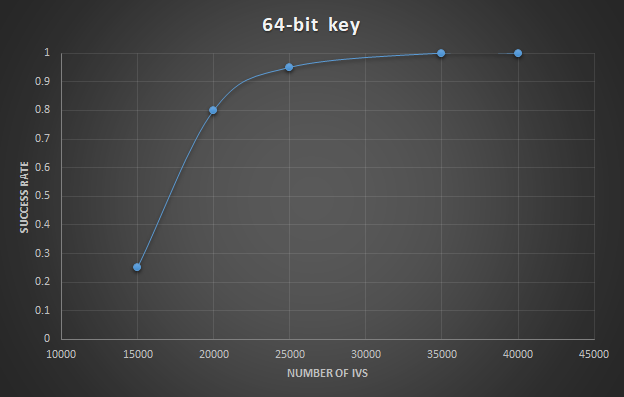
\includegraphics[width=1.0\textwidth]{./images/64bit.png} 
        \caption{Success rate of cracking 64-bit WEP by number of captured IVs}
    \end{minipage}\hfill
    \begin{minipage}{0.45\textwidth}
        \centering
        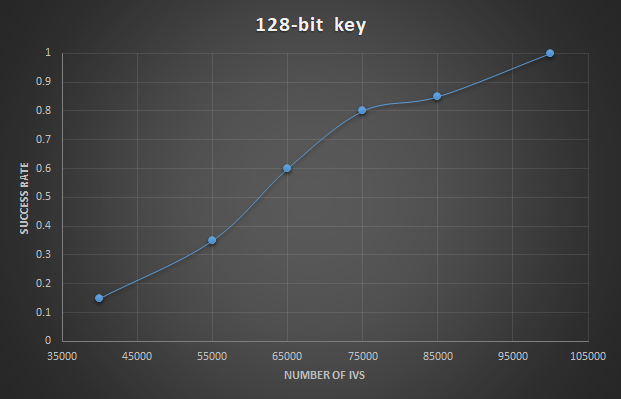
\includegraphics[width=1.0\textwidth]{./images/128bit.png}
        \caption{Success rate of cracking 128-bit WEP by number of captured IVs}
    \end{minipage}
\end{figure}

A major focus in \cite{mainPaper} is the time it takes for this attack to work, and as mentioned in the title, they claim to be able to do it in under 1 minute. Although we were not able to obtain that kind of speed for 128-bit keys, it is possible that this 1 minute mark is obtainable with a more powerful attack machine, as well as having more devices on the victim network generating traffic (as opposed to our single device). The time taken by IV target number can be seen in the graph below.

\begin{figure}[H]
 	\centering
    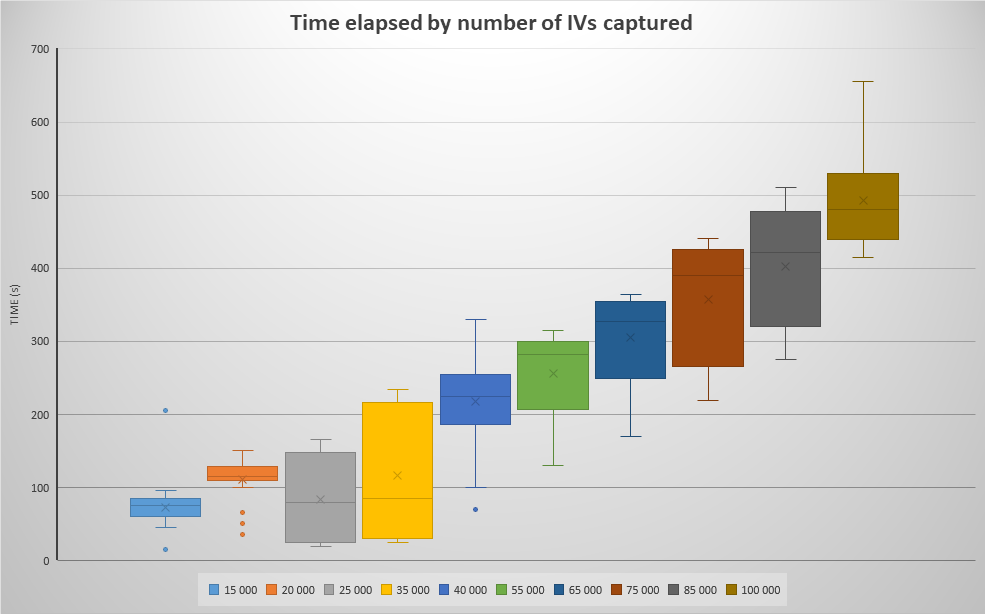
\includegraphics[width=0.5\textwidth]{./images/unknown-3.png}
    \caption{Time elapsed to obtain desired number of IVs}
\end{figure}

The entire process of sending the packets, sniffing the packets, handling the file IO operations, was handled by a very old laptop with 4GB of RAM, and an AMD E-350 laptop CPU with 2 core and 2 threads. This caused the CPU usage to be at 100\% at all times (Figure 3 and Figure 4), but the RAM barely being used (Figure 4). This leads us to believe that faster times could have been reached on better hardware, but we did not have the hardware available to test it on. \\

\begin{figure}[H]
 	\centering
    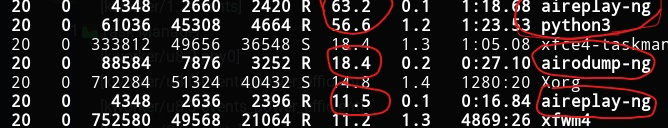
\includegraphics[width=0.5\textwidth]{./images/top_procs.jpg}
    \caption{Top Processes, highlighting CPU usage}
\end{figure}

\begin{figure}[H]
 	\centering
    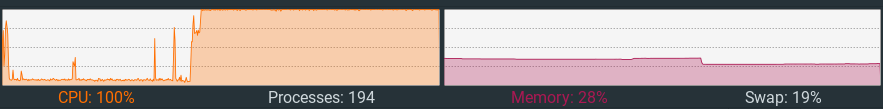
\includegraphics[width=0.5\textwidth]{./images/task_manager_process_view.png}
    \caption{Task Manager}
\end{figure}

This means that deploying this attack on a Raspberry Pi would be possible, there just might be a performance loss in terms of acquiring the desired number of IVs. When it came time to attempt to crack the password, it took, on average, 10 seconds on the laptop. This same process took, on average, 1 second on a modern desktop CPU. The raspberry pi would therefore be capable of cracking the password as well, although it is a task that could be outsourced to a desktop after the packets are captured.



\section{Conclusion}
- Any linux hardware would work, enabling it to be super incognito\\
- Incredibly fast to crack it once enough IVs obtained (less than 1 second in most cases)\\
- Underlying encryption is broken, which is why the attack works so well\\
- Add citations using \cite{klein}\\

- Even though WEP is completely broken, this does not mean that WPA/WPA2 are void of faults. There are compromising attacks, like the KRACK attack (https://www.krackattacks.com/), which are able to decrypt WPA2 and WPA traffic. KRACK does this by exploiting a vulnerability in the 4-way handshake and forcing a nonce re-use by replaying the third message of the 4-way handshake. This goes to show how difficult it is to guarantee 100\% protection for Wi-Fi networks.


% ---------------------------------------- Bibliography Section ---------------------------------------- %
\newpage
% Define the bibliography style to be used, and the bibliography file.
\bibliographystyle{unsrtnat}
\bibliography{sources}{}
\newpage


% Close and Finish Document
\end{document}
\endinput
